\chapter{Introduction}

Initially after the Big Bang, there were one billion and one matter particles for one billion anti-matter particles, which suggests that the current universe should also have abundant anti-matter. However, our current universe is almost entirely built up by matter particles. This is famously known as matter-antimatter asymmetry and is one of the open questions of physics.  A fundamental
difference in the behavior of matter and antimatter, the \textit{CP} violation, is one of the effects
known as Sakharov conditions to explain this asymmetry.\\

The \textit{CP} symmetry is the product of two symmetries: the charge inversion \textit{C}, which
describes the transition of particles into their antiparticles, and the space coordinate
mirroring parity \textit{P}. In 1973, Kobayashi and Maskawa introduced a mechanism to explain \textit{CP} violation in the Standard Model (SM) through the CKM matrix - a mathematical framework describing how quarks change flavors via the weak force.\\

Despite its success, the \textit{CP} violation predicted by the Standard Model is far too small to explain the vast matter-antimatter imbalance. Therefore, new sources of \textit{CP} violation are needed and many New Physics models propose them. Searching for deviations from SM predictions in precision experiments could reveal such new physics and perhaps even explain other open questions, like dark matter.\\

The \textit{CP} violation can be studied experimentally by comparing the decays of particles
and antiparticles. The LHCb experiment is specifically designed for such studies in the
\textit{B} meson region and has already provided substantial results. The analysis to be performed in this study is based on the largest \textit{CP} violation effects
observed on the Run 1 dataset.\\

This analysis is performed on a dataset of reconstructed events of \textit{B} decays and the objective
is to compare the decay rates of 
$B^{+} \to h^{+}h^{+}h^{-}$
and the ones of its antiparticle equivalent
$B^{-} \to h^{-}h^{-}h^{+}$, where $h^{\pm}$ can be pions ($\pi^{\pm}$) or kaons ($K^{\pm}$). The possible decays are:
\begin{itemize}
    \item $B^{+} \to K^{+}K^{+}K^{-}$
    \item $B^{+} \to \pi^{+}K^{+}K^{-}$
    \item $B^{+} \to K^{+}\pi^{+}\pi^{-}$
    \item $B^{+} \to \pi^{+}\pi^{+}\pi^{-}$
\end{itemize}
as well as their corresponding antiparticle decays. Due to the low background level this
analysis focuses on the $B^{+} \to K^{+}K^{+}K^{-}$ decay. In order to recognize and select only events
involving \textit{B} decays, some important physical properties such as momentum, mass and impact parameter are considered. Figure \ref{feynman} shows Feynman diagrams for the $B^{+} \to K^{+}K^{+}K^{-}$ decay.

\begin{figure}[H]
    \centering
    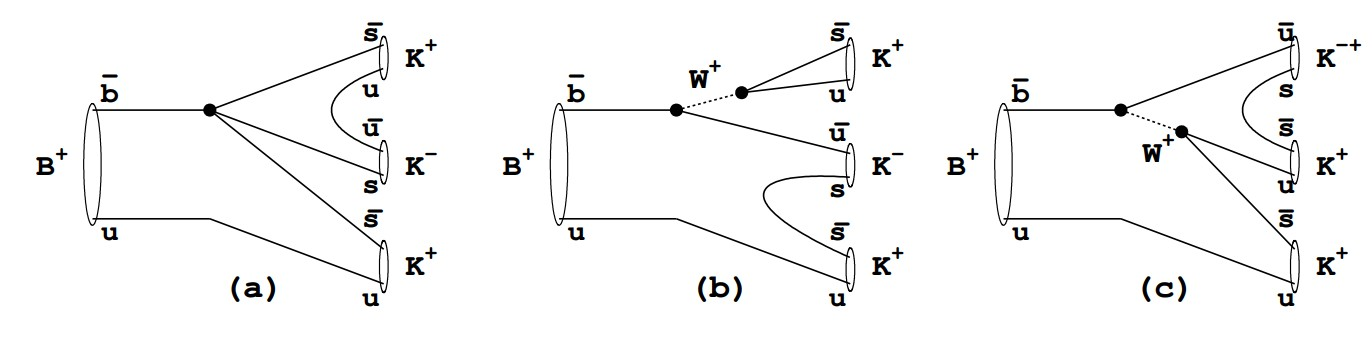
\includegraphics[width=0.8\linewidth]{Figure/1.jpg}
    \caption{Feynman diagrams for $B^{+} \to K^{+}K^{+}K^{-}$ decay: (a) b → s penguin; (b) and (c) b → u trees \cite{feynman}.}
    \label{feynman}
\end{figure}